\section{Chapter 4 : Identification}
The focus of MIDA 1 are \textbf{parametric} identification or learning techniques.
They are the most used and popular identification techniques but many non-parametric techniques are essential for identification ( ex: state-space identification ,spectrum estimation ,unsupervised learning...)\\
Any \textbf{parametric identification technique} is based on a \textbf{five step approach}:
\begin{enumerate}
\item \textbf{Experiment design \& data collection}\\
This step deals with \textbf{designing} the experiment, selecting the \textbf{length N} of the dataset and \textbf{data pre-processing}.
\item \textbf{Selection of a class of parametric models}\\
This steps deals with the selection of \textbf{class} of parametric models $m(\theta)$ where $\theta$ is the unknown parameter vector. Our focus will be on :\\
-\textbf{discrete time}\\
-\textbf{dynamic}\\
-\textbf{linear}\\
-\textbf{time-invariant}\\
systems. As already seen \textbf{ARMAX \& ARMA} are the most general class of models for these systems.
\item \textbf{Selection of a performance index}\\
A function $J(\theta) \geq 0 $ that tells the \textbf{ordering} of different models.
The performance index assesses the \textbf{quality} of a model.\\
The \textbf{prediction error method} is the choice for our performance index:
\[
\boxed{J_N(\theta) = \frac{1}{N} \sum\limits_{t=1}^{N}(y(t)-\hat{y}(t|t-1,\theta))^2}
\]
that represents the \textbf{sample variance} of the prediction error computed on the available dataset of length N.\\
The P.E.M assumes that the ability of a model to make a good prediction of the future is a good \textbf{quality index} for the model.\\
\item \textbf{Optimization}\\
Optimization consists in \textbf{minimizing} $J(\theta)$ with respect to $\theta$ :
$$ \hat{\theta} = argmin_{\theta}\{J(\theta)\}$$ so that $$ m(\hat{\theta}) $$ is the \textbf{optimal model} on the class of models $m(\theta)$.
$$ J_N(\theta) = R^{n_\theta} \rightarrow R^{+}$$
In optimisation 3 different situations can be found:
\begin{itemize}
\item $J(\theta)$ is \textbf{quadratic} function of $\theta$\\
\begin{figure}[H]
 \centering
  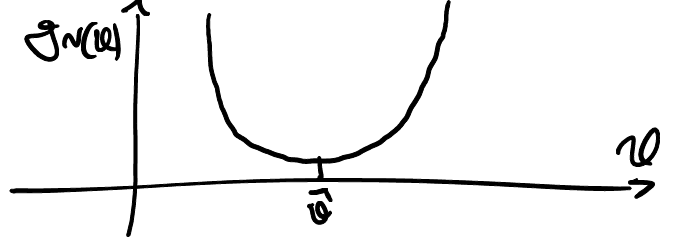
\includegraphics[width=.4\linewidth]{quadratic.png}
\end{figure}
$J_N$ is a \textbf{quadratic} function of $\theta$ : in this case it's usually easy to find the \textbf{global minimum} explicitly.\\
\textbf{AR \& ARX} models are of this kind.
\item $J(\theta) $ is \textbf{not} a quadratic function , \textbf{no local minima}\\
\begin{figure}[H]
 \centering
  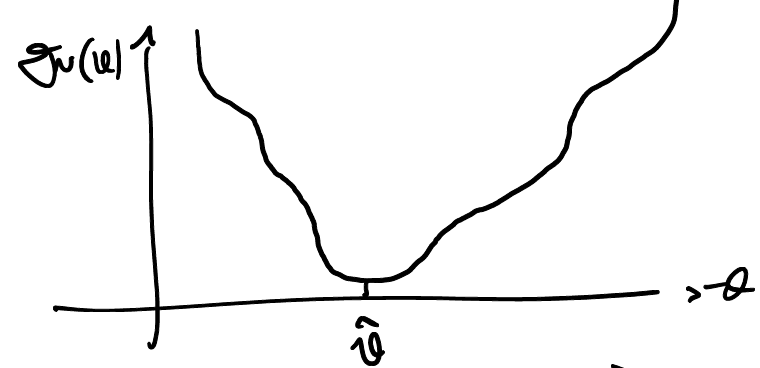
\includegraphics[width=.4\linewidth]{n_quadratic}
\end{figure}
In this case the function has no local minima so the \textbf{unique solution} is guaranteed to be found using an \textbf{iterative algorithm}.\\
\item $J(\theta)$ is \textbf{not} quadratic, \textbf{with local minima}\\
\begin{figure}[H]
 \centering
  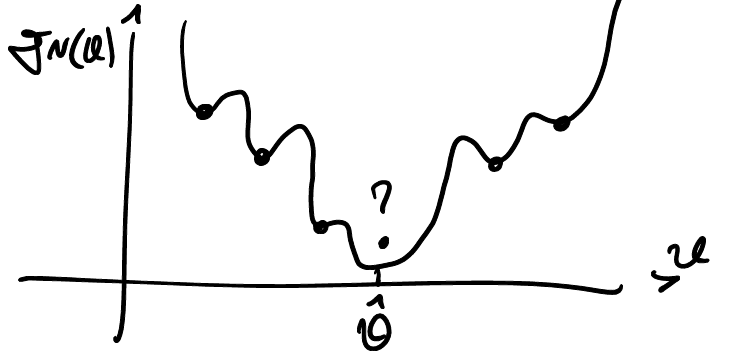
\includegraphics[width=.4\linewidth]{n_quadratic_local}
\end{figure}
In this case the function has local minima so using an \textbf{iterative algorithm} is the best way to find the unique solution which is \textbf{not guaranteed} to be found.\\
\textbf{ARMAX \& ARMA} models are of this kind.
\end{itemize}
\item \textbf{Validation}\\
The validation step checks if $m(\hat{\theta})$ can be considered a \textbf{valid} model for our purposes. Usually a technique called \textbf{cross-validation} is used.
\end{enumerate}

\newpage
\subsection{Identification of ARX models}
Given an available dataset of length N :
$$ \{ u(1),u(2),...,u(N)\}$$
$$ \{ y(1),y(2),...,y(N)\}$$
An the model class \textbf{ARX(m,p+1)}:
$$ y(t) = \frac{B(Z)}{A(Z)}u(t-1)+\frac{1}{A(Z)}e(t) , e(t) \sim WN(0,\lambda^2)$$
where
 $ \theta = \begin{bmatrix}
                a_1  
                ...  
                a_m 
                b_0  
                ...  
                b_p 
             \end{bmatrix}^T$ 
is the \textbf{parameter vector} of dimension $n_{\theta} = m+p+1$.
\begin{description}
\item[Remark]\hfill\\
Using \textbf{k=1} is not a restriction but the \textbf{most general} case of an ARX. If the system has $k > 1$ we will find out during the identification process.
\end{description}
\subsubsection{Loss function: Least Squares}
The loss function for the ARX models is the \textbf{P.E.M.}:
\[
\boxed{J_N(\theta) = \frac{1}{N} \sum\limits_{t=1}^{N}(y(t)-\hat{y}(t|t-1,\theta))^2}
\]
The predictor for the model , deriving it from the  general ARMAX model, is :
$$ \hat{y}(t|t-1;\theta) = \frac{B(Z)}{1}\cdot 1\cdot u(t-1)+ (1-A(Z))y(t)$$
\[
\boxed{\hat{y}(t|t-1;\theta) = b_0u(t-1)+...+b_pu(t-p-1)-a_1y(t-1)-...-a_my(t-m)}
\]

where we can define the \textbf{data vector}:
$$ \phi = \begin{bmatrix}
                -y(t-1),  
                ...  
                -y(t-m) ,
                
                u(t-1),
                ...  
                u(t-p-1) 
             \end{bmatrix}^T$$ 

so $\hat{y}(t|t-1) = \phi(t)^T \theta$ , a linear function of $\theta$. Substituting in the loss function:
$$ J_N(\theta)= \frac{1}{N} \sum\limits_{t=1}^{N}(y(t) - \phi(t)\theta)^2$$
A \textbf{quadratic} function is obtained so the \textbf{unique solution} can be found explicitly using a minimization method.To find the minimum we differentiate wrt to the parameter vector $\theta$ : 
$$ \frac{\partial{J_N(\theta)}}{\partial \theta} = 0$$
$$ \frac{\partial{J_N(\theta)}}{\partial \theta} = \frac{2}{N}\sum\limits_{t=1}^{N}\phi(t)(y(t)-\phi(t)^T\theta)$$

$$ (\sum\limits_{t=1}^{N} \phi(t)\phi(t)^T)\theta = \sum\limits_{t=1}^{N} y(t) \phi
(t)$$
Assuming that the $n_{\theta} $ x $ n_{\theta} $ matrix $\sum\limits_{t=1}^{N}\phi(t)\phi(t)^T$ matrix is \textbf{non singular } and thus \textbf{invertible}:
\[
\boxed{\hat{\theta}_N= (\sum\limits_{t=1}^{N}\phi(t)\phi(t)^T)^{-1}(\sum\limits_{t=1}^{N}y(t)\phi(t))}
\] 
This is the \textbf{explicit} solution of the ARX identification problem also known as \textbf{Least Squares}

\subsubsection{Example}
Consider a dataset of length N=10 and 
$$ y(t) = \frac{b}{1+aZ^{-1}}u(t-1)+\frac{1}{1+aZ^{-1}}e(t), e(t) \sim WN(0,\lambda^2)$$
an ARX(1,1) general model class.
Assuming that the process is in canonical representation ( $|a|<1$ must hold).
The predictor of the model is :
$$ \hat{y}(t|t-1)= \frac{B(Z)}{1}u(t-1)+\frac{1-A(Z)}{1}e(t)$$
\[
\boxed{\hat{y}(t|t-1)=bu(t-1)-ay(t-1)}
\]
and $\theta= [a,b]^T$.\\
\begin{description}
\item[Method 1]\hfill\\

The loss function is :
$$ J_{10}(\theta) = \frac{1}{10}\sum\limits_{t=1}^{10}(y(t) - bu(t-1)+ay(t-1))^2$$
\begin{description}
\item[Remark]\hfill\\
Since we don't have data points for t=0 , starting at time t=1 doesn't allow us to compute $-bu(0)+ay(0)$ so a modified version of the performance index is used:
\[
\boxed{J_N(\theta)= \frac{1}{N-h}\sum\limits_{t=h+1}^{N}(y(t)-\hat{y}(t|t-1))^2}
\]
where $h=max\{m,p+1\}$
\end{description}
In our case $h=max(1,1)=1$ so 
$$ J_{10}(\theta) = \frac{1}{9}\sum\limits_{t=2}^{10}(y(t) - bu(t-1)+ay(t-1))^2$$
To obtain the best parameter vector $\to \frac{\partial{J_{10}(\theta)}}{\partial{\theta}} = 0$ where $\theta = [a,b]^T$ :
\[ \frac{\partial{J_{10}(\theta)}}{\partial{\theta}} =
  \begin{cases}
        \frac{\partial{J_{10}(\theta)}}{\partial{a}} = \frac{2}{9} \sum\limits_{t=2}^{10}(y(t)-bu(t-1)+ay(t-1))\cdot y(t-1) = 0  \\
    		\frac{\partial{J_{10}(\theta)}}{\partial{b}} = \frac{2}{9} \sum\limits_{t=2}^{10}(y(t)-bu(t-1)+ay(t-1))\cdot (-u(t-1)) = 0  
  \end{cases}
\]
Which can be rewritten as : 
$$ 			\begin{bmatrix}
          \sum\limits_{t=2}^{10}y(t-1)^2 & -\sum\limits_{t=2}^{10}y(t-1)u(t-1) \\
          -\sum\limits_{t=2}^{10}y(t-1)u(t-1) & \sum\limits_{t=2}^{10}u(t-1)^2
             \end{bmatrix} \cdot
             \begin{bmatrix}
          	   a\\
               b
             \end{bmatrix}= 
             \begin{bmatrix}
          -\sum\limits_{t=2}^{10}y(t-1)y(t) \\
          \sum\limits_{t=2}^{10}y(t)u(t-1) 
             \end{bmatrix}
              $$ 
so
$$ 	\begin{bmatrix}
          	   \hat{a}_{10}\\
               \hat{b}_{10}
             \end{bmatrix} =
			\begin{bmatrix}
		\sum\limits_{t=2}^{10}y(t-1)^2 & -\sum\limits_{t=2}^{10}y(t-1)u(t-1) \\
		-\sum\limits_{t=2}^{10}y(t-1)u(t-1) & \sum\limits_{t=2}^{10}u(t-1)^2	
			\end{bmatrix}^{-1}
			\begin{bmatrix}
			-\sum\limits_{t=2}^{10}y(t-1)y(t) \\
			\sum\limits_{t=2}^{10}y(t)u(t-1)
\end{bmatrix}					             
             $$ 
\item[Method 2]\hfill\\
Consider the predictor $\hat{y}(t|t-1)= bu(t-1)+ay(t-1) $ and the available data.
Assuming that the predictor makes the \textbf{perfect prediction} on the measured data :
\[ 
\begin{cases}
 -ay(1)+bu(1)=y(2) \\
 -ay(2)+bu(2)=y(3) \\
 ...\\
 -ay(9)+bu(9)=y(10)
\end{cases}
\]
Which can be separated into two matrices:
$$ 	\Phi = \begin{bmatrix}
          	  -y(1) & u(1) \\
              -y(2) & u(2) \\
              ...   & ...  \\
              -y(9) & u(9) 
             \end{bmatrix}
            Y= \begin{bmatrix}
             y(2)\\
             y(3) \\
             ... \\
             y(10)
             \end{bmatrix}$$
Obtaining a \textbf{linear} system of 9 equations and 2 unknowns :
\[
\boxed{\Phi \cdot \theta = Y} 
\]
---------------------------------------------------------------------------------------------------
\begin{description}
\item[Remark]\hfill\\
\begin{itemize}
\item \textbf{Undetermined linear system}\\
Number of unknowns > number of equations $\to$ \textbf{infinite solutions}
\item \textbf{Square linear system}\\
Number of unknowns = number of equations $\to$ \textbf{1! solution}
\item \textbf{Over determined linear system}\\
Number of unknowns < number of equations $\to$ \textbf{No solutions!}
\end{itemize}
\end{description}
---------------------------------------------------------------------------------------------------
\\Unfortunately our case is the last one with no solutions! In this case a \textbf{least squares} (\textbf{approximate)} solution can be found using the square matrix  :\\ $ \Phi \theta = Y \to \Phi^T \Phi \theta = \Phi^T Y $
\[
\boxed{ \hat{\theta} = [\Phi^T \Phi]^{-1} \Phi^T Y} 
\]
where $ [\Phi^T \Phi]^{-1} \Phi^T = \Phi^{+} $ is the \textbf{pseudo inverse} of $\Phi$. By creating the matrices above we obtain the \textbf{same} result for 
$\hat{\theta}$
\end{description}

\subsubsection{Example 2}
Assume a dataset of 5 points collected from an SSP with zero mean.
$ y(1)= \frac{1}{2}, y(2) = 0 , y(3) = -1 , y(4) = -\frac{1}{2}, y(5)= \frac{1}{4}$
and we want to make a prediction $ \hat{y}(6|5) $
\begin{description}
\item[1.Build the model]\hfill\\
We selected a class of model \textbf{AR(1)} (reason discussed further on ).
$$ y(t) = ay(t-1)+e(t) e(t) \sim WN(0,\lambda^2)$$ is our $ m(\theta) $.
Transforming $ \to y(t) = \frac{1}{1-aZ^{-1}}e(t) $ which is in canonical representation if $|a<1|$.
The corresponding k=1 predictor is $$ \hat{y}(t|t-1) =\frac{C(Z) - A(Z)}{C(Z)}y(t) \to \hat{y}(t|t-1) = ay(t-1) $$ with \textbf{performance index}:
$$ J_5(a)= \frac{1}{4} \sum\limits_{t=2}^{5} (y(t) -ay(t-1))^2$$
After some easy computation we find that $ J_5(a) = \frac{1}{4}[\frac{3}{2}a^2 -\frac{3}{4}a+\frac{21}{16}]$ which is the measure to be \textbf{minimized}:
$$ \frac{\partial{J_5(a)}}{\partial{a}}= \frac{1}{4}[3a-\frac{3}{4}]=0$$
Which has solution $$ \hat{a}_5=\frac{1}{4}$$ So best model identified in AR(1) class is : 
\[
\boxed{y(t) = \frac{1}{1-\frac{1}{4}Z^{-1}}e(t)}
\]
\item[2.Compute prediction]\hfill\\
$ \hat{y}(6|5) = \frac{1}{4}y(5) = \frac{1}{16}$
\item[3. First remark]\hfill\\
Is $\hat{a}= \frac{1}{4}$ fine?Yes , it hold the condition that $|a|<1$.\\
What if $\hat{a}=4$? In that case we have to find the \textbf{canonical form} of the system.
\item[4. Second remark]\hfill\\
The variance of the white noise $\lambda^2$ is not required for the model and prediction estimation.  If we wanted to estimate also $\lambda^2$ and not only a (which still is the most important parameter to estimate):
$$ \lambda^2 = var[e(t)] \to var[\epsilon(t)]$$
Using an \textbf{approximate estimation} using the 5 available data points :
$$ \hat{\lambda_{5}^2} = J_5(\hat{a}_5)$$
\end{description}
\newpage
\subsection{Identification of ARMAX models}
While ARX model estimation relies on \textit{least squared method} , ARMAX model estimation relies on \textbf{maximum likelihood}.\\
Given the available N-long data vector \textbf{u} and \textbf{y} , the model class is $m(\theta): y(t) = \frac{B(Z)}{A(Z)}u(t-1) + \frac{C(Z)}{A(Z)}e(t)$ where 
$$A(Z) = 1+ ...+a_mZ^{-m} $$
$$B(Z) = b_0+...+b_pZ^{-p}$$
$$C(Z) = 1+...+c_nZ^{-n}$$
and working under the hypothesis that $\frac{C(Z)}{A(Z)}$ is in \textbf{canonical representation} $\to$ \textbf{ARMAX(m,n,p+1)} where k=1 is \textbf{not} a restriction but indeed the \textbf{most general case}.\\
Using the P.E.M. approach : $$ \hat{\theta} = argmin_{\theta}=\{J_N(\theta)\}$$
with performance index $$J_N(\theta) = \frac{1}{N} \sum\limits_{t=1}^{N}(y(t)-\hat{y}(t|t-1,\theta))^2$$ where the parameter vector has dimension $n_{\theta}=m+n+p+1$: $$ \theta =[a_1,...,a_m,b_0,...b_p,c_1,...,c_m]^T $$
Since k=1 $\epsilon(t)= e(t)= \frac{A(Z)}{C(Z)}y(t)-\frac{B(Z)}{C(Z)}u(t-1)$ so the performance index $$ J_N(\theta) = \frac{1}{N} \sum\limits_{t=1}^{N}(\frac{A(Z)}{c(Z)}y(t) -  \frac{B(Z)}{C(Z)}u(t-1))^2$$
This performance index is now an issue as it kills the optimisation : C(Z) is a \textbf{non-linear} function of $\theta$ so it is not a quadratic function of $\theta$. So the \textbf{minimization} requires an \textbf{iterative approach}.

\subsubsection{Loss function :Maximum Likelihood Method}
The \textbf{iterative} loss function of ARMAX models starts from an initial condition $\theta^1 \to \theta^2...\to \hat{\theta}_N$  until a final solution is reached
\begin{figure}[H]
 \centering
  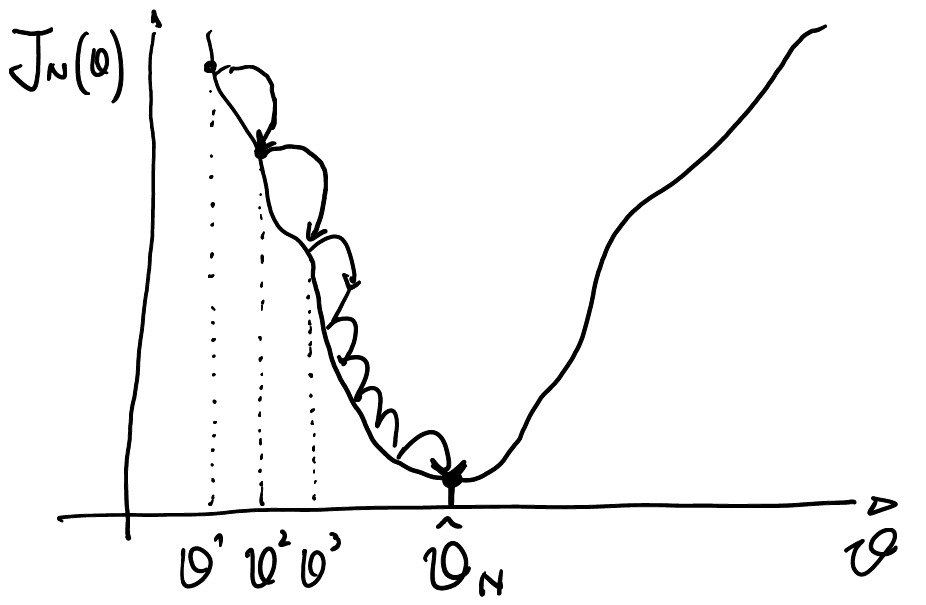
\includegraphics[width=.5\linewidth]{iterative.png}
\end{figure}
Unfortunately usually $J_N(\theta)$ has lots of \textbf{local minima}:
\begin{figure}[H]
 \centering
  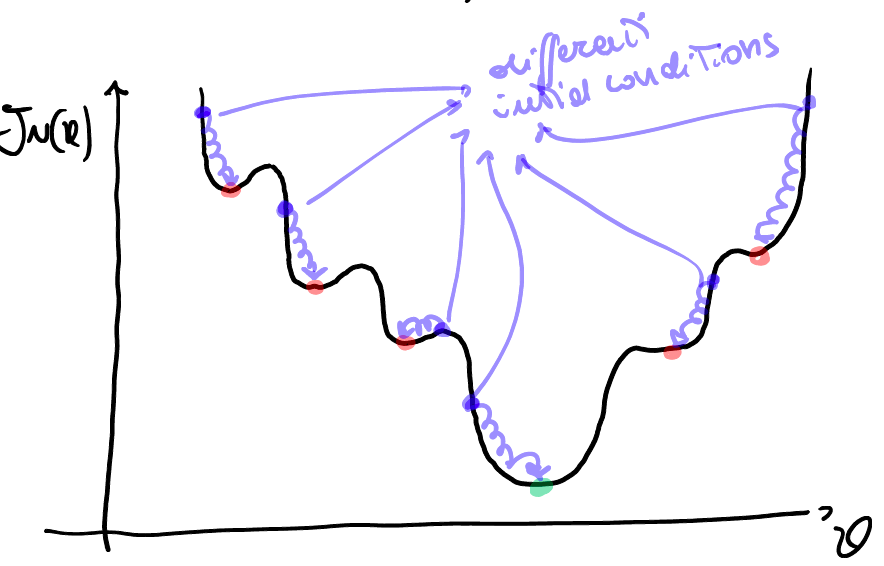
\includegraphics[width=.5\linewidth]{iterative_minima.png}
\end{figure}
To attenuate this disturbance many \textbf{different} initial conditions  $\theta^1$ should be used , each time trying to reach the best solution. The problem is that there is no \textbf{theoretical guarantee} that solution converges to the global minimum.\\
The key problem for iterative methods is building the \textbf{step} : 
$$ \theta^i \to \theta^{i+1} $$
The basic idea is to compute the \textbf{local quadratic approximation} of $J_N(\theta)$ around the point $\theta^i$ and \textbf{minimize the local approximation} using the \textbf{Newton method} 
\begin{figure}[H]
 \centering
  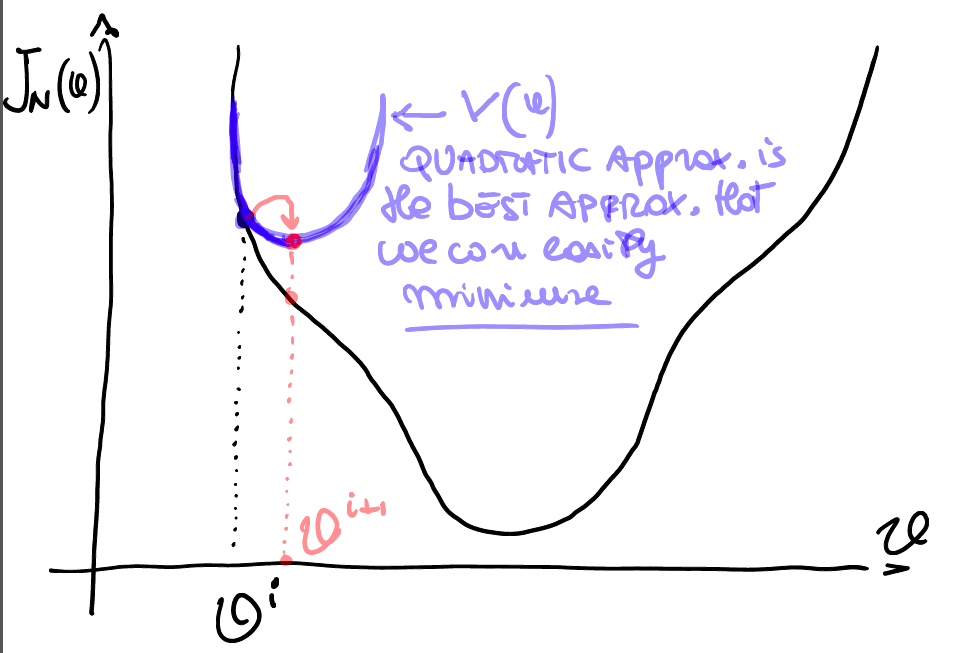
\includegraphics[width=.6\linewidth]{newton.png}
\end{figure}
Using \textbf{Taylor's expansion} around $\theta^i$:
$$\gamma(\theta)=  J_N(\theta^i) + \left[\left. \frac{\partial{J_N(\theta)}}{\partial{\theta}}\right|_{\theta^i} \right](\theta-\theta^i)+ \frac{1}{2}(\theta-\theta^i)^T\left[\left. \frac{\partial^2{J_N(\theta)}}{\partial^2{\theta}}\right|_{\theta^i} \right](\theta-\theta^i)...$$
Minimizing the function $\gamma(\theta) \to \frac{\partial{\gamma(\theta)}}{\partial{\theta}}=0$:
$$  \left[\left. \frac{\partial{J_N(\theta)}}{\partial{\theta}}\right|_{\theta^i} \right] + \frac{1}{2} \cdot 2 \left[\left. \frac{\partial^2{J_N(\theta)}}{\partial^2{\theta}}\right|_{\theta^i} \right] (\theta - \theta^i) =0$$

\[
 \boxed{\theta  = \theta^i -  \left[\left. \frac{\partial^2{J_N(\theta)}}{\partial^2{\theta}}\right|_{\theta^i} \right]^{-1} \cdot  \left[\left. \frac{\partial{J_N(\theta)}}{\partial{\theta}}\right|_{\theta^i} \right]}
\]
Where the first is matrix is the inverse of the second order derivative ( \textbf{Hessian Matrix} ) of $J_N(\theta)$ around $\theta^i$ and the second matrix is the first order (\textbf{Gradient Vector}) of $J_N(\theta)$ around $\theta^i$.
\begin{itemize}
\item \textbf{Gradient vector}\\
 $$\frac{\partial{J_N(\theta)}}{\partial{\theta}} = \frac{2}{N}\sum\limits_{t=1}^{N}\epsilon(t) \cdot \frac{\partial{\epsilon(t)}}{\partial{\theta}}$$
 \item \textbf{Hessian matrix}\\
$$\frac{\partial^2{J_N(\theta)}}{\partial^2{\theta}}= \frac{2}{N}\sum\limits_{t=1}^{N} \frac{\partial{\epsilon(t)}}{\partial{\theta}} \cdot \frac{\partial{\epsilon(t)}}{\partial{\theta}}^T + \frac{2}{N}\sum\limits_{t=1}^{N}\epsilon(t)\frac{\partial^2{\epsilon(t)}}{\partial{\theta^2}}$$
Which can be approximated to :
$$\frac{\partial^2{J_N(\theta)}}{\partial^2{\theta}}= \frac{2}{N}\sum\limits_{t=1}^{N} \frac{\partial{\epsilon(t)}}{\partial{\theta}} \cdot \frac{\partial{\epsilon(t)}}{\partial{\theta}}^T $$
The approximation holds because of three reasons:
\begin{enumerate}
\item \textbf{Reason}\\
We can compute the Hessian using only $\frac{\partial{\epsilon(t)}}{\partial{\theta}}$ without the burden of computing $\frac{\partial^2{\epsilon(t)}}{\partial{\theta}^2} $
\item \textbf{Reason}\\
Since $\epsilon(t,\theta)= y(t) - \hat{y}(t|t-1;\theta)$ notice that $\frac{\partial^2{\epsilon(t)}}{\partial{\theta}^2} $ does \textbf{not} depend on y(t) but only on $\hat{y}(t|t-1;\theta) \to y(t-1),y(t-2),...$.\\
Moreover if $\theta^i$ is close to the \textbf{optimum} , $\epsilon(t;\theta) \approx e(t)$. So under these assumptions $\epsilon(t;\theta^i)$ and $\left. \frac{\partial^2{\epsilon(t)}}{\partial{\theta}^2} \right|_{\theta^i}$ are \textbf{uncorrelated} (orthogonal).
\item \textbf{Reason}\\
By neglecting the second Hessian term we can guarantee that the approximation is \textbf{semi-definite positive } $(\geq 0)$
\end{enumerate}
\begin{figure}[H]
 \centering
  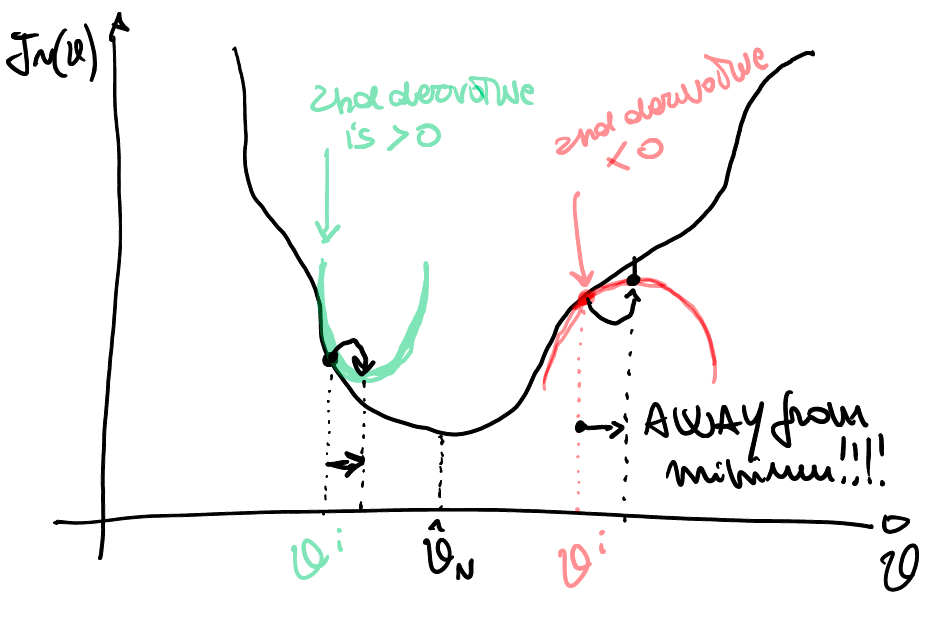
\includegraphics[width=.6\linewidth]{hessian}
\end{figure}
In conclusion the approximation \textbf{guarantees} that the updating step always goes in the \textbf{right direction!}
\end{itemize}
The final updating rule is :
\[
\boxed{\theta^{i+1} = \theta^i - \left[ \sum\limits_{t=1}^{N} \frac{\partial \epsilon(t;\theta^i)}{\partial{\theta}} \cdot \frac{\partial \epsilon(t;\theta^i)^T}{\partial{\theta}} \right]^{-1} \cdot  \left[ \sum\limits_{t=1}^{N} \epsilon(t;\theta) \cdot \frac{\partial \epsilon(t;\theta^i)}{\partial{\theta}} \right]}
\]

How to calculate $\frac{\partial \epsilon(t;\theta)}{\partial{\theta}}$?\\
$$\epsilon(t,\theta)= \frac{A(Z)}{C(Z)}y(t) - \frac{B(Z)}{C(Z)}u(t-1)$$
$$ \epsilon(t,\theta)= \frac{1+a_1Z^{-1}+...+a_mZ^{-m}}{1+c_1Z^{-1}+...+c_nZ^{-n}} y(t) - \frac{b_0+...+b_pZ^{-p}}{1+c_1Z^{-1}+...+c_nZ^{-n}}u(t-1)$$
where $\theta =[a_1,...,a_m,b_0,...,b_p,c_1,...,c_n]^T$. Deriving for each element in the parameter vector:
\begin{description}
\item[Parameters a]\hfill\\
$$ \frac{\partial{\epsilon(t,\theta)}}{\partial{a_1}}= \frac{Z^{-1}}{C(Z)}y(t)=\frac{1}{C(Z)}y(t-1) = \alpha(t-1) \text{defined!}$$
$$ \text{...}$$
$$ \frac{\partial{\epsilon(t,\theta)}}{\partial{a_m}}= \frac{Z^{-m}}{C(Z)}y(t)=\frac{1}{C(Z)}y(t-m) = \alpha(t-m) \text{defined!}$$
\item[Parameters b]\hfill\\
$$ \frac{\partial{\epsilon(t,\theta)}}{\partial{b_0}}= -\frac{1}{C(Z)}u(t-1)= \beta(t-1) \text{defined!}$$
$$ \text{...}$$
$$ \frac{\partial{\epsilon(t,\theta)}}{\partial{b_p}}= \frac{Z^{-p}}{C(Z)}u(t-1)=\frac{1}{C(Z)}u(t-p-1) = \beta(t-p-1) \text{defined!}$$
\item[Parameters c]\hfill\\
$$ (1+c_1Z^{-1}+...+c_nZ^{-n})\epsilon(t,\theta)=A(Z)y(t)-B(Z)u(t-1)$$
$$ Z^{-1}\epsilon(t,\theta)+C(Z)\frac{\partial{\epsilon(t,\theta)}}{\partial{c_1}}=0$$
$$ \frac{\partial{\epsilon(t,\theta)}}{\partial{c_1}} = - \frac{1}{C(Z)}\epsilon(t-1,\theta)= \gamma(t-1) \text{defined!}$$
$$ \text{...}$$
$$ \frac{\partial{\epsilon(t,\theta)}}{\partial{c_n}} = - \frac{1}{C(Z)}\epsilon(t-n,\theta)= \gamma(t-n) \text{defined!} $$
\end{description}
In conclusion :
\[
\boxed{\frac{\partial{\epsilon(t,\theta)}}{\partial{\theta}}= [\alpha(t-1),...,\alpha(t-m),\beta(t-1),...,\beta(t-p-1),\gamma(t-1),...,\gamma(t-n)]^T}
\]
We obtain a vector m+n+p+1 of \textbf{defined signals}.\\
A \textbf{filtering scheme} can used to compute the vector:
\begin{figure}[H]
 \centering
  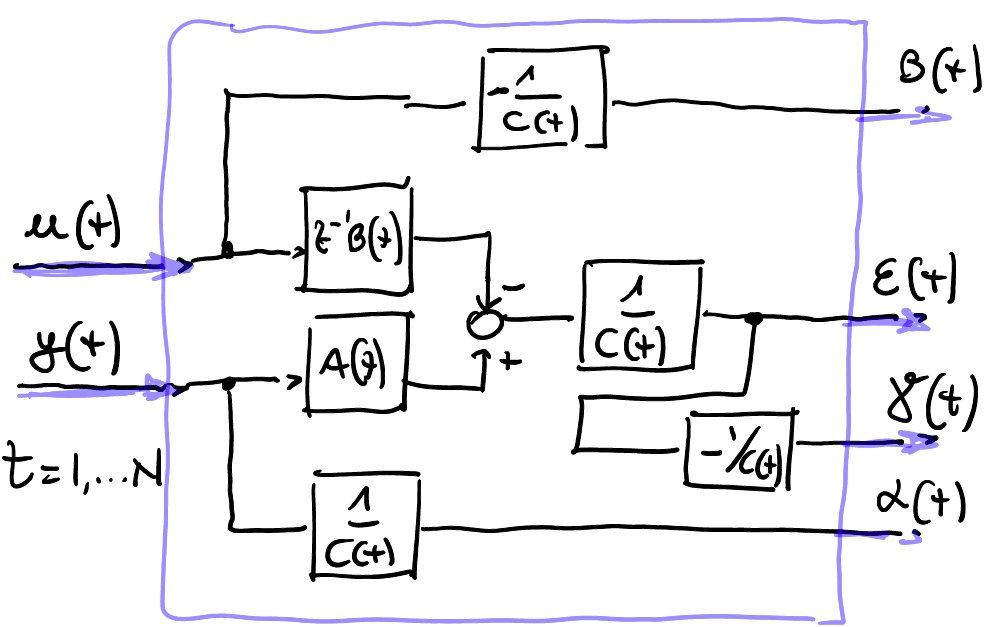
\includegraphics[width=.6\linewidth]{filtering}
\end{figure}

\subsubsection{Possible issues}
\begin{enumerate}
\item The Hessian approximation might not be \textbf{invertible} $\to$ solution : add term $\delta I$
\item The polynomial $C(Z)^i$ might have roots \textbf{outside} the unit circle. The resulting filtering is not asymptotically stable $\to$ solution : canonical form
\end{enumerate}







\subsubsection{Possible updating rules}
There are different \textbf{updating rules} which have all the same general expression : 
\[
\boxed{\theta^{i+1} = \theta^i - \bigcirc  \cdot \left[ \frac{\partial{J_N(\theta)}}{\partial{\theta}}\right]}
\] 

\begin{itemize}
\item \textbf{Gradient method}\\
$$ \bigcirc = \mu $$  $\mu$ is a scalar number called \textbf{step}.
Characteristics :\\
+ simplest method\\
+ correct direction \textbf{guaranteed}\\
- slow when near to minimum\\
- sensitive to choice of $\mu$ (too small = slow, too big = instability)\\
This method is the backpropagation rule in NN.
\item \textbf{Newton method}\\
$$ \bigcirc = \text{Inverse of hessian matrix of performance index} $$ 
\item \textbf{Quasi- Newton method}\\
$$ \bigcirc = \text{Inverse of} \geq \text{approximation of the Hessian} $$ 
This is the one seen in 4.2.1.\\
Has all the positive aspects of Newton method ( variable step tuned to the specific point of optimisation )but can guarantee the right direction of the step.\\
To avoid the singularity of matrix $ \sum\limits_{t=1}^{N} \frac{\partial \epsilon(t;\theta^i)}{\partial{\theta}} \cdot \frac{\partial \epsilon(t;\theta^i)^T}{\partial{\theta}} $ usually $\delta I$ is added where $\delta$ is a small number and $I$ the identity matrix. 
\end{itemize}